
\documentclass[parskip]{cs4rep}

\usepackage{graphicx}

\usepackage{url}

\begin{document}

\title{An LLVM based compiler from Objective-C to Dalvik Virtual Machine}

\author{Stanislav Manilov}

% to choose your degree
\degree{Computer Science and Mathematics}

% to choose your report type
\project{4th Year Project Report}

\date{\today}

\abstract{
The rapidly growing mobile app market of today, and the need of developers for cross-platform tools justify the creation of a system that can translate iPhone applications to Android ones. Such a system would need to have an Objective-C to Dalvik binary compiler, an Android version of the Cocoa API, and an interface translating module. The goal of this project is to produce a compiler, using LLVM as a foundation. A successful implementation would produce applications that are comparable in size and performance with Java written equivalents. At the time of writing, the system is 60\% complete, with the plan of having it 100\% complete within two weeks and using the rest of the semester to write the dissertation.
}

\maketitle

\tableofcontents

%\pagenumbering{arabic}

\chapter{Introduction}

\section{Background}

Today we observe a rapidly growing mobile applications market \cite{P1}
that induces equally fast growing demand for high-quality and reliable development
tools. In 2011 the market generated a revenue of \$5.5 bn \cite{P1},
which is estimated to be 6.5 \% of the value of the desktop software market
(please, see Figure ~\ref{fig:softwareMarket2011}). This illustrates the significance of the mobile applications market.

\begin{figure}[h!]
  \label{fig:softwareMarket2011}
  \caption{Software market size in 2011 \cite{P1} \cite{P2} \cite{P3}.}
  \centering
    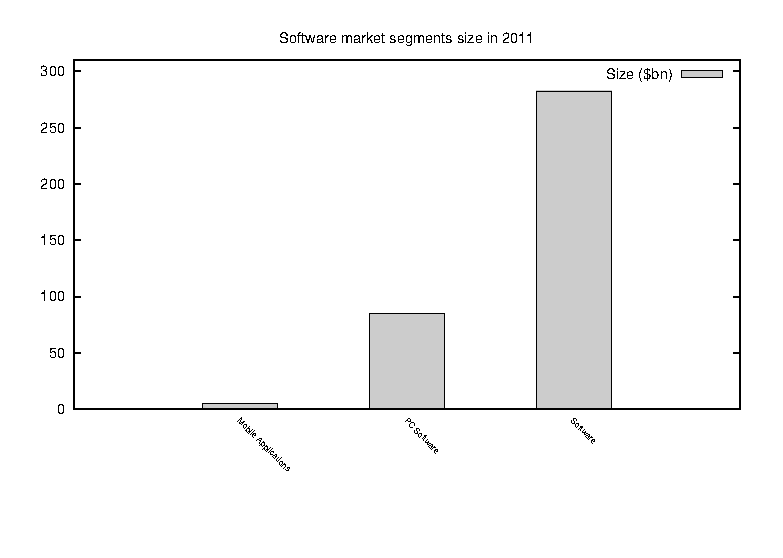
\includegraphics[width=1.0\textwidth]{markets}
\end{figure}

A main challenge for mobile app developers is producing and maintaining cross-platform applications. Although there are already plenty of tools that address writing such applications (please, see Table ~\ref{tab:crossPlatformTools}), there are three main problems with them:

\begin{itemize}
\item
all of them require learning additional languages (e.g. HTML, JavaScript, or
Lua),
\item
most of them violate the Apple SDK Agreement \cite{P5} \cite{P6} by
producing apps originating from disallowed languages, and
\item
none of them can deal with automatic porting of already existing code that was
originally written for a specific platform.
\end{itemize}

\begin{table}
    \label{tab:crossPlatformTools}
    \caption{Comparison of popular cross-platform mobile tools \cite{P4}}
    \centering
    \begin{tabular}{ | l | p{4.4cm} | p{2.6cm} | p{3cm} |}
    \hline
    Name & Required Knowledge & Cost & Since \\ \hline
    Sencha Touch & HTML, CSS, JavaScript & Free & November 2010 \\ \hline
    jQuery Mobile & HTML, CSS, jQuery & Free & October 2010 \\ \hline
    Tiggzi & HTML, CSS, JavaScript & \$0 - \$180 pm & Unknown \\ \hline
    AppMakr & HTML, CSS & \$79 pm & January 2010 \\ \hline
    iBuildApp & HTML, CSS & \$10 pm & 2010 \\ \hline
    Widgetbox & HTML, CSS & \$25 - \$100 pm & October 2010 \\ \hline
    foneFrame & HTML, CSS, JavaScript & \$0 - \$59 & Unknown \\ \hline
    phoneGap & HTML, CSS, JavaScript & Free & August 2008 \\ \hline
    Corona & Lua & \$200 - \$350 py & December 2009 \\ \hline
    \end{tabular}
\end{table}

These points justify the creation of a compiler that can take the source code of
an iPhone application written in Objective-C and produce an equivalent Android
application. However, there are a couple of major issues with this idea:
firstly, the libraries used for iPhone development - Cocoa API - are proprietary
and thus can not be compiled for Android, and secondly, interface guidelines for
the two platforms differ and thus interfaces can not be literally translated.
Fortunately, there is a community effort to solve the first problem - the
GNUStep project. And while the interface guidelines differ, they are
specific enough to make the detection and translation of idioms possible.

This discussion outlines two of the three major components that a system of the required type must have: a version of the Cocoa API, compiled for the Android platform, and an interface translation module. The third necessary component is, of course, a compiler core that can translate the actual program logic. As building the whole system is an ambitious task for an honours project, it was decided that the effort would be concentrated on the program logic component. If successful, this project can be built upon, adding the additional critical components for creating a complete, automatic porting facility.

\section{Goals}

As outlined in the background section, the goal of this project is to build a system, using which, an Objective-C code can be compiled to a Dalvik executable and can be ran on an Android emulator or an actual Android based smart phone. Essential properties of the system are:
\begin{itemize}
\item
correctness: the produced program should be working as described by the source code;
\item
speed: the time to build a typical program should be acceptable (in the order of minutes at worst).
\end{itemize}

In addition to these, it is desirable that the resulting system has the following properties:

\begin{itemize}
\item
performance of produced code: the produced program should be reasonably fast (same order of magnitude), when compared to an identical program, written in Java and built using the standard tool chain (Android Development Kit);
\item
size of produced code: the size of the produced program should be reasonably small, when compared to an identical program, written in Java and built using the standard tool chain.
\end{itemize}

The system should be available as a command-line tool. Different options should be available to specify properties (e.g. name or entry point) of the program to be built. Building a graphical user interface or an interactive system is not in the scope of this project.

The Objective-C programs that the compiler must be able to handle are command-line programs that do not depend on external libraries.

\chapter{Approach}

\section{Design}

Before the commencing of the work on the project, it was agreed that the best approach is to base the system on the LLVM compiler infrastructure. There are multiple advantages that come with building upon LLVM:
\begin{itemize}
\item
Firstly, LLVM comes with clang - a complete frontend for languages based on the C programming language. This includes Objective-C, so basing Objective-Droid on LLVM would remove the need of producing front-end components like a parser or a lexer.
\item
Secondly, LLVM comes with a powerful middle end that contains a wide range of optimizations \cite{P7}. Including them in Objective-Droid would be highly beneficial to the quality of the output, while at the same time, it would be infeasible and unnecessary to duplicate all the work of implementing these optimizations.
\item
Thirdly, using an established compiler infrastructure as a foundation would provide an interface that developers are already used to, at no additional effort. This would reduce the learning curve for users of Objective-Droid and let them feel more confident about using the tool.
\item
Fourthly, building a backend for LLVM by the guidelines would allow it to be contributed to the project, thus all, or parts of Objective-Droid can be given back to the compiler developer community easier than if it is being developed from scratch.
\end{itemize}
Thus, the first essential component of the Objective-Droid system is the LLVM backend. The target code was decided to be smali code, as there are already assembling tools for it that produce Dalvik binaries.

The second essential component is a packager that given the smali code assembles it, packages it, and signs the package. This would allow the package to be installed and tested on an emulator or a phone.

The final component of the Objective-Droid system is a wrapper program or a script that automates the whole process of compiling, packaging, and possibly installing the program on a phone. This script would be useful for testing, but is not mandatory.

For a summary of the design, please see Figure ~\ref{fig:design}.

\begin{figure}[htp]
  \label{fig:design}
  \caption{Overall design of the Objective-Droid system.}
  \centering
    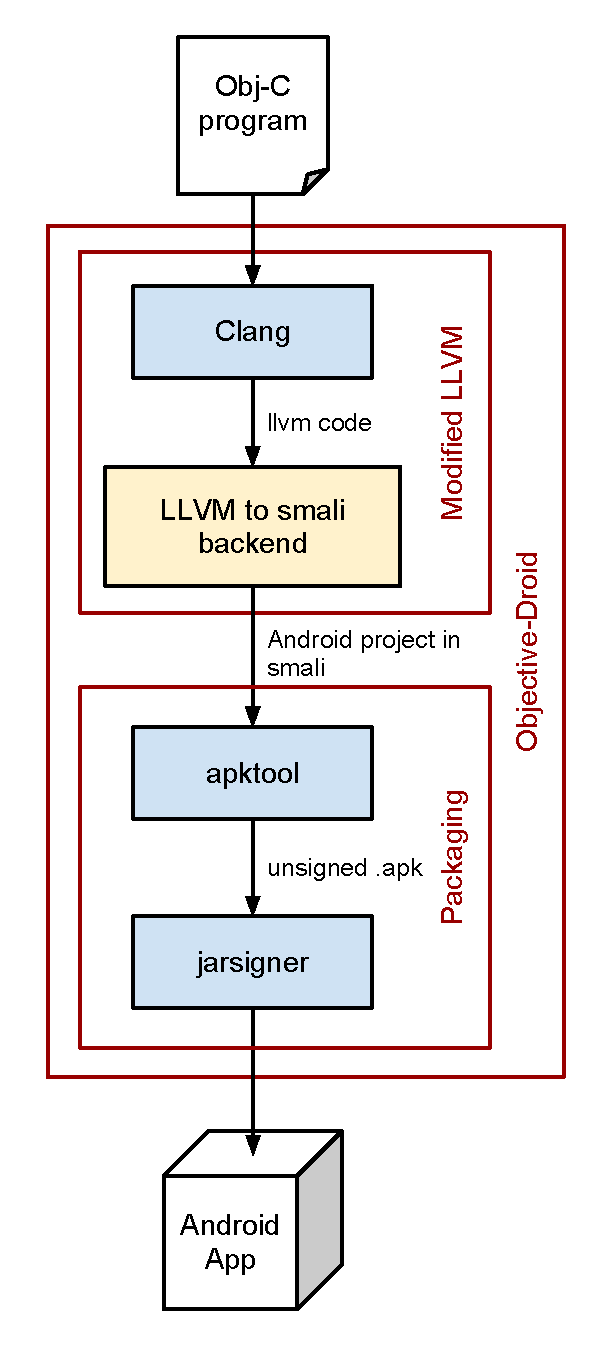
\includegraphics[width=0.6\textwidth]{design}
\end{figure}

\section{Implementation}

\subsection{File structure}

As apparent from the design outline, the most integral part of the project is building the LLVM backend. This required familiarising with the conventions that are accepted within the LLVM community for undertaking such work, and understanding the general structure of a backend.

An LLVM backend needs to be implemented as a subclass of the TargetMachine class \cite{P8}. Depending on the features of the target architecture, the implementation needs to provide a suite of files. E.g. if MIPS is the target architecture, the implementation needs to provide files that describe: the instructions, the registers, the interface for JIT compilation, etc. On the other hand, if the target is not a real architecture, but rather a high-level language, the implementation can be as simple as a single class. This is the case of the backend that produces C++ code.

The initial approach taken when developing the Objective-Droid backend was to follow the general structure and provide separate classes for the different functions of the backend. However, this was decided to be overly complicated, especially when compared to the approach of the C++ backend. It was argued that the code that the backend has to produce - smali code - is not actual machine code, so it does not need many of the classes that a code for a real architecture would require (e.g. an assembler definition).

Thus, for the main part of the project the backend was developed in a single monolithic class. Still, attempting to use the full target class hierarchy was not a waste of time, as it provided an insight of how the LLVM project works - an insight that was helpful later.

The decision to write the whole backend as a single class provoked the danger of bad maintainability. Thus, during development, effort was put towards writing simpler and cleaner code at first, and then optimising the common parts of it. Also, comments were put as documentation, as general comments, and as specific comments explaining complicated code. The overall result was readable code that is easy to understand for a newcomer to the project.

\subsection{{\tt Target} class}

The main class of the implementation inherits the {\tt ModulePass} class of LLVM. The {\tt ModulePass} is typically used for passes that manipulate the whole program, thus it serves the needs of the Objective-Droid backend. This makes the {\tt runOnModule} method to be the entry point of the class. This method is given a description of the program in a {\tt Module} object as an argument and returns {\tt false} on success.

The implementation of the {\tt runOnModule} method simply builds a corresponding Android {\tt Activity} class by iterating over the global variables and functions of the {\tt Module}, and translating them to static fields and to static methods, respectively. The boiler-plate code for the class includes a start up method - {\tt onCreate} - which is a standard way of starting up an Android {\tt Activity}. It invokes the translation of the main function of the supplied Objective-C code, and calls the typical {\tt finish} method that terminates the program.

The functions are translated by iterating over the instructions in them and translating each one in separately. It was found that for most instructions this is trivial, and others were either simply translated to a series of instructions (as in the case of comparison instructions) or emulated by a dedicated external library. This approach would result in a slightly lower performance of the output program, but ensures good performance of compilation and simplicity of the compiler.

\chapter{Progress}

\section{Up to now}

At the time of writing, the system is 60\% complete. This includes 75\% of the instructions being translated, and a prototype of the packaging script being produced.

Two months were spent in researching about LLVM and initialising a separate backend component. The next two months were spent in incremental implementation of instructions, alongside thorough testing to ensure the correctness of each translation. This method proved useful, as it caught defects in implementation, notably in instructions that required to be emulated by a sequence of other instructions (e.g. the 'set on compare' instructions). During this period a code base of benchmark programs emerged and will be used after the project is complete for its evaluation.

\section{Left to do}

The programming work that remains to be done is:
\begin{itemize}
\item
translating global variables as static fields
\item
translating the remaining 25\% of the instructions
\item
supporting multiple file compilation
\item
cleaning up the source code
\item
adding missing documentation
\end{itemize}

When this is done, the supporting scripts need to be updated and polished, after which the system will be evaluated against the benchmark code base. Finally, the dissertation would be written up and submitted.

The following milestones are scheduled:
\begin{itemize}
\item
February 10 / academic week 4 - have a full-featured version of the system
\item
February 24 / academic week 6 - finish most of the testing and have a foundation for the final report
\item
March 10 / academic week 8 - finish first draft of the report and submit it for review
\item
March 24 / academic week 10 - implement feedback from the review and submit a final draft of the report for review
\item
April 8 / academic week 12 - prepare a draft presentation and submit it for review; submit final report
\item
April 22 - finalise presentation and submit for review
\item
week starting April 29 - Present
\end{itemize}

% use the following and \cite{} as above if you use bibtex
% otherwise generate bibtem entries

\bibliographystyle{plain}
\bibliography{mybibfile}

\end{document}